\documentclass[10pt,letterpaper,spanish,twoside]{report}

\usepackage{practica}
\usepackage{graphicx}
\usepackage{float}
\DeclareGraphicsExtensions{.bmp,.png,.pdf,.jpg}
\newcommand{\docdate}{
  \vspace{2em}
   \begin{flushright}
     Ciudad de México. \datedayname~\today.
   \end{flushright}
  \vspace{2em}
}

\begin{document}
\docdate

\begin{center}
 \textsc{\asignatura}\vspace{.2em}
\end{center}

\textsc{Manual del profesor}

\textsc{Práctica 5. Aplicación de filtros Chebyshev tipo 1 y 2 digitales para la detección de frecuencia cardiaca.}

\textsc{Objetivo:} Aplicar los conocimientos sobre el diseño de filtros digitales Chebyshev tipo I y II para la detección de la frecuencia cardiaca mediante el procesamiento de señal de sonidos de Korotkoff.

\textsc{Actividades}
\begin{enumerate}
 \item Se descarga el archivo 'sonidos.npz' de http://drives.news/google247, que contiene datos de los sonidos de Korotkoff obtenidos con un micrófono marca Nihon Kohden, modelo: TK-701T y con No. de serie:00652
 \item En la figura~\ref{contexto:Korotkoff} se muestra la gráfica de la señal de los sonidos de Korotkoff.\\Se puede observar que al inicio de la señal se observa interferencia que es ocasionada por algún artefacto de movimiento, seguida de las cinto fases de los sonidos de Korotkoff y por último, la etapa del silencio.
 \begin{figure}[H]
 	\centering
 	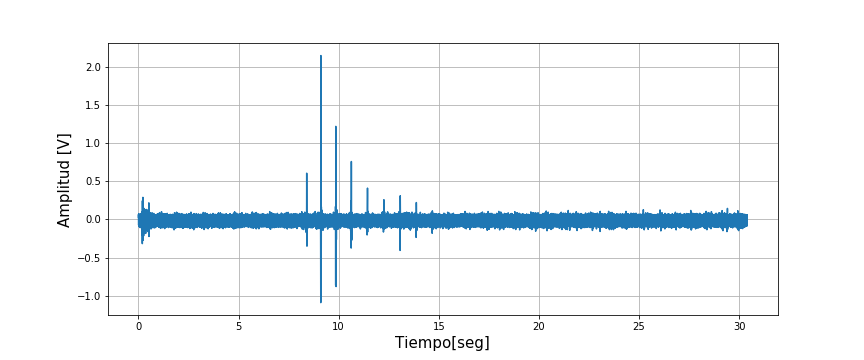
\includegraphics[scale=0.4]{sounds.PNG}
 	\caption{Señal de sonidos de Korotkoff}
 	\label{contexto:Korotkoff}
 \end{figure}
 \item Se obtiene la FFT de la señal original para observar la interferencia, sabemos que el contenido espectral de los sonidos de Korotkoff se encuentra entre 20-300 Hz (rango audible), en la figura~\ref{contexto:FFT_sounds} es posible observar que la señal de interés tiene un contenido espectral entre 20-50 Hz.
 \begin{figure}[H]
	\centering  
	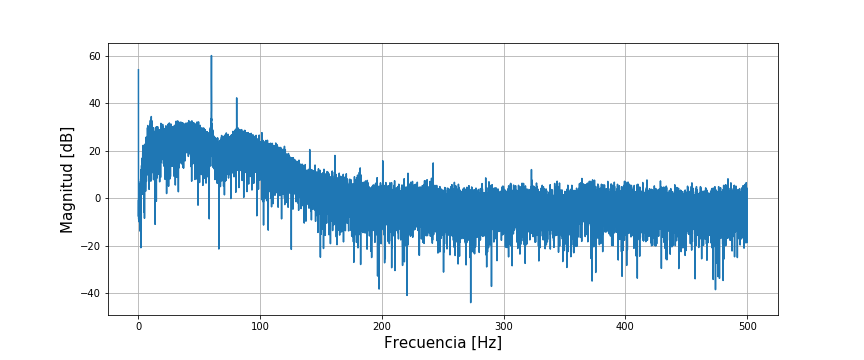
\includegraphics[scale=0.4]{FFT_sounds.PNG}
	\caption{FFT de los sonidos de Korotkoff}
	\label{contexto:FFT_sounds}
 \end{figure}
 \item Para el diseño del filtro Chebyshev tipo I se sugiere utilizar frecuencias de corte entre 23 y 45 Hz, en la figura~\ref{contexto:RF_C1S} se muestra la caracterización de la respuesta en frecuencia del filtro.
 \begin{figure}[H]
	\centering
	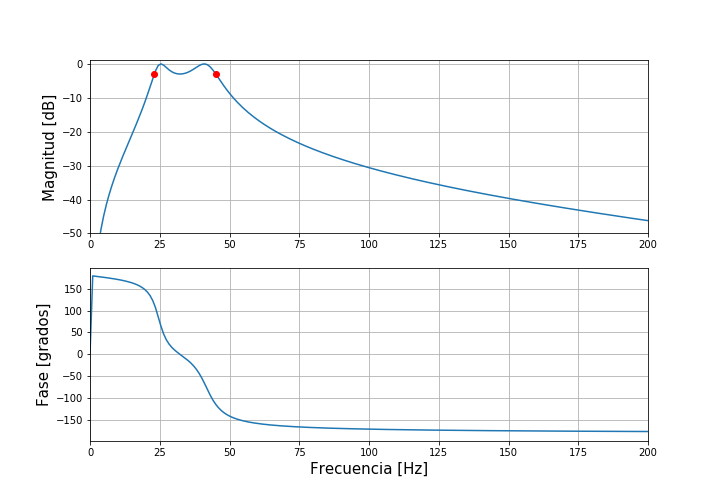
\includegraphics[scale=0.4]{RF_C1S}
	\caption{Caracterización de la Respuesta en frecuencia del filtro pasa banda\\Chebyshev tipo I orden 2}
	\label{contexto:RF_C1S}
 \end{figure}
 \begin{enumerate}
 	\item Es posible observar que las frecuencias de corte se encuentran exactamente en 23 y 45 Hz, esto es debido a que en la función cheby1 que fue utilizada se asignó un valor de rp de 3dB que es la ondulación máxima permitida por debajo de la máxima ganancia en la banda de paso.
 	\item En la figura~\ref{contexto:FFT_C1S} se muestra la FFT de la señal filtrada, es posible observar que la señal fue filtrada correctamente de acuerdo a las frecuencias de corte establecidas.
 \end{enumerate}
 \begin{figure}[H]
 	\centering
 	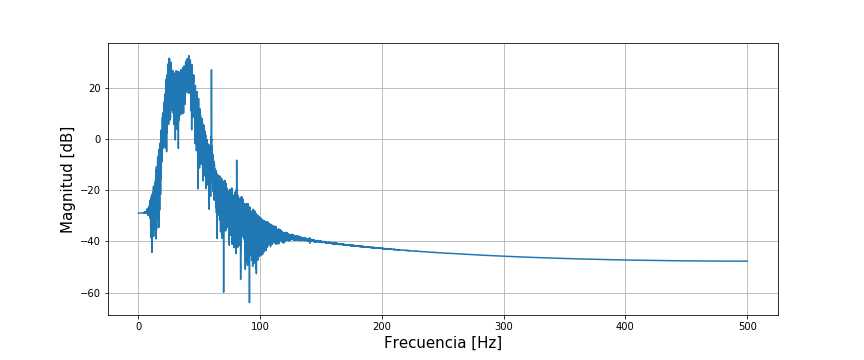
\includegraphics[scale=0.4]{FFT_C1S.PNG}
 	\caption{FFT de la señal filtrada con filtro Chebyshev tipo I}
 	\label{contexto:FFT_C1S}
 \end{figure}
 \item En el diseño del filtro Chebyshev tipo II se sugiere utilizar frecuencias de corte entre 20 y 55 Hz, en la figura~\ref{contexto:RF_C2S} se muestra la caracterización de la respuesta en frecuencia del filtro.
 \begin{figure}[H]
 	\centering
 	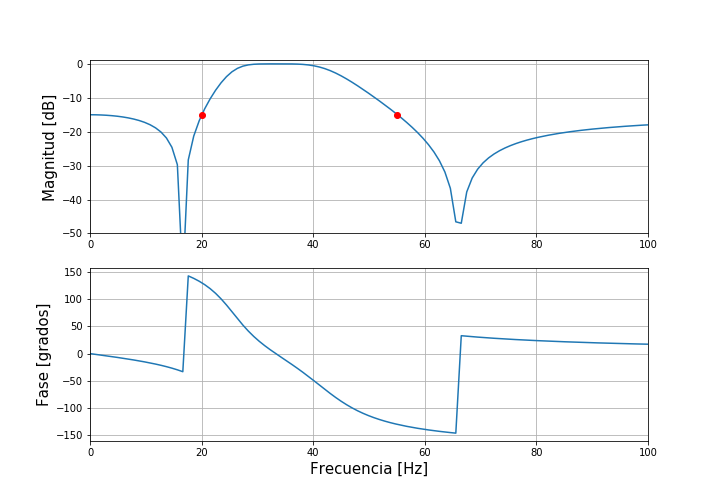
\includegraphics[scale=0.4]{RF_C2S.png}
 	\caption{Caracterización de la respuesta en frecuencia del filtro\\Chebyshev tipo II orden 2}
 	\label{contexto:RF_C2S} 	
 \end{figure}
 \begin{enumerate}
 	\item En la figura~\ref{contexto:FFT_C2S} se muestra la FFT de la señal filtrada, se observa que las frecuencias de corte que fueron elegidas se encuentran en -15 dB esto se debe al valor asignado en rs en la función cheby2, que es la atenuación mínima requerida en la banda de rechazo, este valor fue elegido de manera que filtrara correctamente la señal.
 \end{enumerate}
 \begin{figure}[H]
 	\centering
 	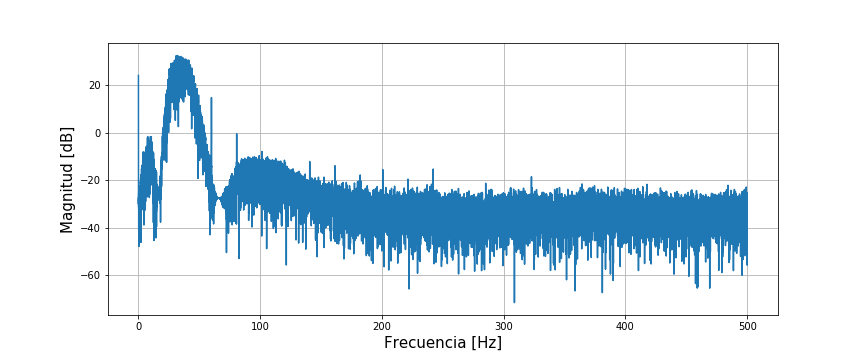
\includegraphics[scale=0.4]{FFT_C2S.PNG}
 	\caption{FFT de la señal filtrada con Chebyshev tipo II orden 2}
 	\label{contexto:FFT_C2S}
 \end{figure}
 \item Para la obtención de la frecuencia cardiaca se lleva a cabo el siguiente proceso, se creó una función que lo realizara el cual puede ser revisado en el script.
 \begin{itemize}
 	\item Obtener la envolvente de la señal 
 	\item Encontrar la posición de los picos
 	\item Obtener el tiempo transcurrido entre dos picos y obtener la frecuencia
 \end{itemize}
 \begin{enumerate}
 	\item En la figura~\ref{contexto:Frec1} se puede observar el proceso anterior para la señal filtrada con Chebyshev tipo I, se especifico un umbral para los picos de 0.14 V y se obtuvo una frecuencia cardiaca de 85 lat$/$min.
 	\begin{figure}[H]
 		\centering
	 	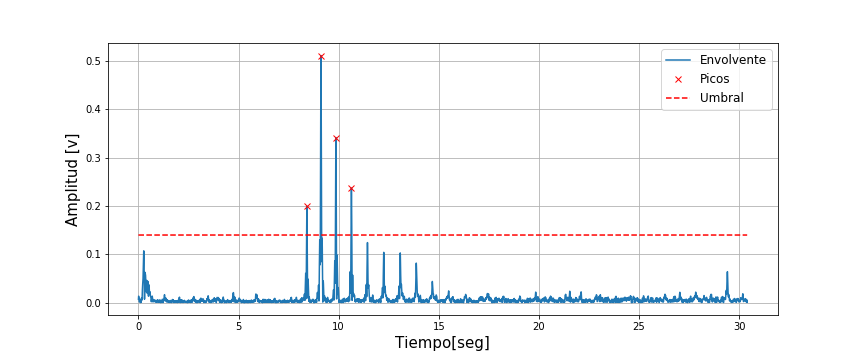
\includegraphics[scale=0.5]{frec1.PNG}
 		\caption{Envolvente de la señal filtrada con Chebyshev tipo I}
	 	\label{contexto:Frec1}
 	\end{figure}
 	\item De igual forma para la señal filtrada con Chebyshev tipo II en la figura~\ref{contexto:Frec2} se obseva la envolvente de la señal, se obtiene la misma frecuencia cardiaca con la diferencia que se utiliza un umbral de 0.13 V.
 	\begin{figure}[H]
 		\centering
 		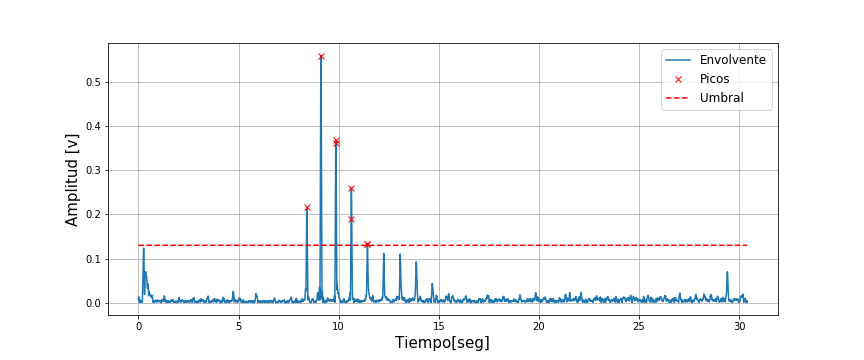
\includegraphics[scale=0.5]{frec2.PNG}
 		\caption{Envolvente de la señal filtrada cin Chebyshev tipo II}
 		\label{contexto:Frec2}
 	\end{figure}
 \end{enumerate}
\end{enumerate}

%\textsc{Nota}
%\vspace{2em}
\vfill
\begin{flushright}
\textsc{Elaboró:\\
Ma. del Rosario Aguilar Cruz\\
Enrique Mena Camilo}
\end{flushright}

\end{document}